
\begin{frame}
  \frametitle{About CMake}

        \begin{itemize}
          \item Open-source application for 'managing the build process' of a software package
          \item CMake is available on all major platforms (Linux, Windows, MacOS, ...) 
          \item Supports source directory trees that depend on multiple libraries
          \item CMake is a script language that includes almost all basic programming language elements
          \item CMake generates a native build environment for the OS it is executed on
          \item Supports in-place and out-of-place builds
          \item Can generate project files for various IDEs (Visual Studio, Xcode, Eclipse, ...)
          \item Has a mechanism to locate libraries in the OS
          \item 'Easy' to enable/disable optional components of a software package ($\rightarrow$ modular builds)
        \end{itemize}
\end{frame}

\begin{frame}
  \frametitle{Features of CMake}

        \begin{itemize}
          \item Saves a lot of time when building for different OSs 
          \item Easier to combine source code written in different languages 
          \item Easier to specify different build options 
          \item Widely used in many open-source packages
          \item Makes it easier to integrate third-party libraries
          \item cmake-gui as a graphical tool to help beginners and explore build options 
          \item ccmake to explore build options on the console 
          \item CDash as a built-in testing system and dashboard 
          \item CTest as a packaging system for the different operating systems 
        \end{itemize}

\end{frame}

\begin{frame}
  \frametitle{Software Packages that use CMake}
  \vspace{-1cm}

  \begin{columns}

    \column{0.5 \textwidth} {

      \begin{block}{Part of the Kitware Family}
        Used for building:
        \begin{itemize}
          \item VTK 
          \item ParaView 
        \end{itemize}
      \end{block}
      \begin{center}
      
\includegraphics[width=0.4 \textwidth]{img/kw-logo.png}
    \end{center}
    }
    \column{0.5 \textwidth} {
      \begin{block}{Open Source Libraries}
        \begin{itemize}
          \item Bullet Physics Enginge 
          \item CGAL 
          \item LAPACK 
          \item MikTeX 
          \item OGRE  
          \item OpenSceneGraph  
          \item Qt  
          \item Many solver packages (Eigen, Super-LU, ...)
          \item FeatFloWer  
          \item Feat3  
          \item ...  
        \end{itemize}
      \end{block}
    }
\end{columns}
\end{frame}

%\begin{frame}
%  \frametitle{Software Packages that use CMake}
%  \begin{tikzpicture}[remember picture,overlay]
%    \tikzset{shift={(current page.center)}}
%
%    \node[text width=8cm] (C1) at (-6.8, 2.5) {
%      \begin{block}{Part of the Kitware Family}
%        Used for building:
%        \begin{itemize}
%          \item VTK 
%          \item ParaView 
%        \end{itemize}
%      \end{block}
%    };
%
%    \node[text width=8cm] (C2) at (5,-1.6) {
%      \begin{block}{Open Source Libraries}
%        \begin{itemize}
%          \item Bullet Physics Enginge 
%          \item CGAL 
%          \item LAPACK 
%          \item MikTeX 
%          \item OGRE  
%          \item OpenSceneGraph  
%          \item Qt  
%          \item Many solver packages (Eigen, Super-LU, ...)
%          \item FeatFloWer  
%          \item Feat3  
%          \item ...  
%        \end{itemize}
%      \end{block}
%    };
%
%%    \node[text width=8cm] (C3) at (0,8) {
%%      \begin{block}{CMake}
%%        \begin{itemize}
%%          \item Script language to control the building process
%%          \item Generates a wide range of specific build files
%%        \end{itemize}
%%      \end{block}
%%    };
%%
%%    \node[text width=8cm] (C4) at (0,7) {
%%      \begin{block}{ParaView}
%%        \begin{itemize}
%%          \item VTK visualization by GUI
%%          \item Scripting via Python
%%          \item Extension by plugins
%%        \end{itemize}
%%      \end{block}
%%    };
%
%\end{tikzpicture}
%\end{frame}


\begin{frame}[fragile]
  \frametitle{CMake Simple Example}
  \vspace{-0.5cm}

  \begin{block}{CMakeLists.txt}
\begin{verbatim}
  cmake_minimum_required (VERSION 2.8)

  project(HelloWorld)

  set(mySources main.cpp)

  add_executable(HelloWorld ${mySources})

\end{verbatim}
\end{block}

\begin{center}
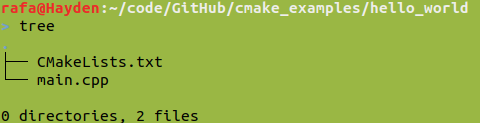
\includegraphics[width=0.8 \textwidth]{img/source-tree.png}
\end{center}

\end{frame}

\begin{frame}
  \frametitle{Out-Of-Source-Builds}
  \begin{itemize}
    \item Source files are in a different directory than the binary files 
  \end{itemize}

  \begin{center}
    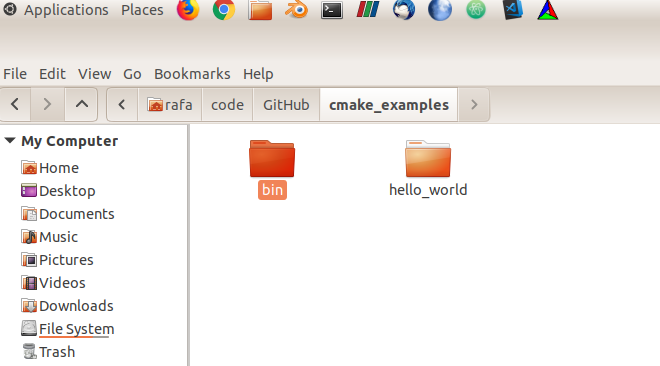
\includegraphics[width=0.8 \textwidth]{img/source-bin.png}
  \end{center}

\end{frame}

\begin{frame}
  \frametitle{Simple CMake Build Procedure}
  \begin{center}
    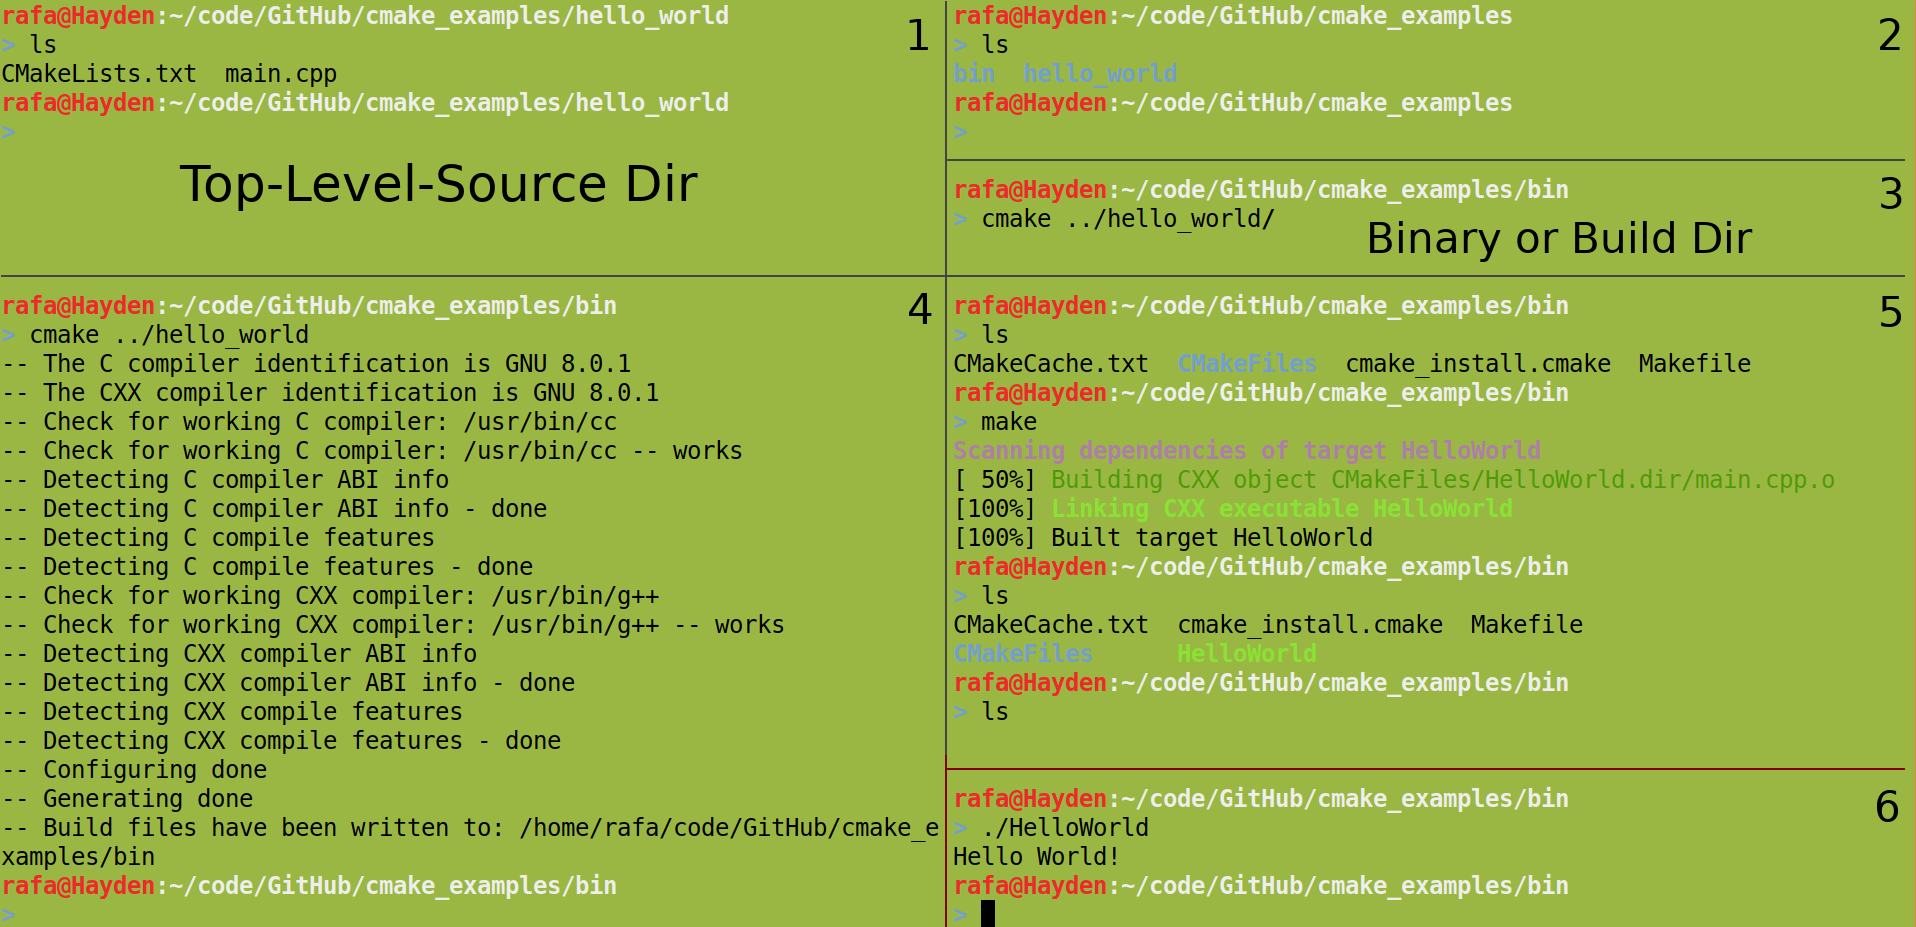
\includegraphics[width=\textwidth]{img/cmake-command-line.png}
  \end{center}
\end{frame}

\begin{frame}
  \frametitle{Simple CMake Build Procedure II}

    \begin{itemize}
      \item Searches for a file 'CMakeLists.txt' in the top level source directory as entry point 
      \item Two step process: 
      \begin{itemize}
        \item Configure step: parses the CMakeLists.txt files and stores information in CMake cache
        \item Generation of the OS specific build files based on the CMakeLists.txt
      \end{itemize}
      \item CMake Syntax: https://cmake.org/cmake/help/v3.13/manual/cmake-language.7.html
      \item For more complex source trees, subdirectories can be added with the \texttt{add\_subdirectory()} command
      \item Subdirectories added via \texttt{add\_subdirectory()} then need their own CMakeLists.txt file
      \item For each directory that contains a CMakeLists.txt a corresponding directory is created in the build directory tree
    \end{itemize}

\end{frame}

\begin{frame}[plain]
  \frametitle{CMake GUI}

  \begin{center}
    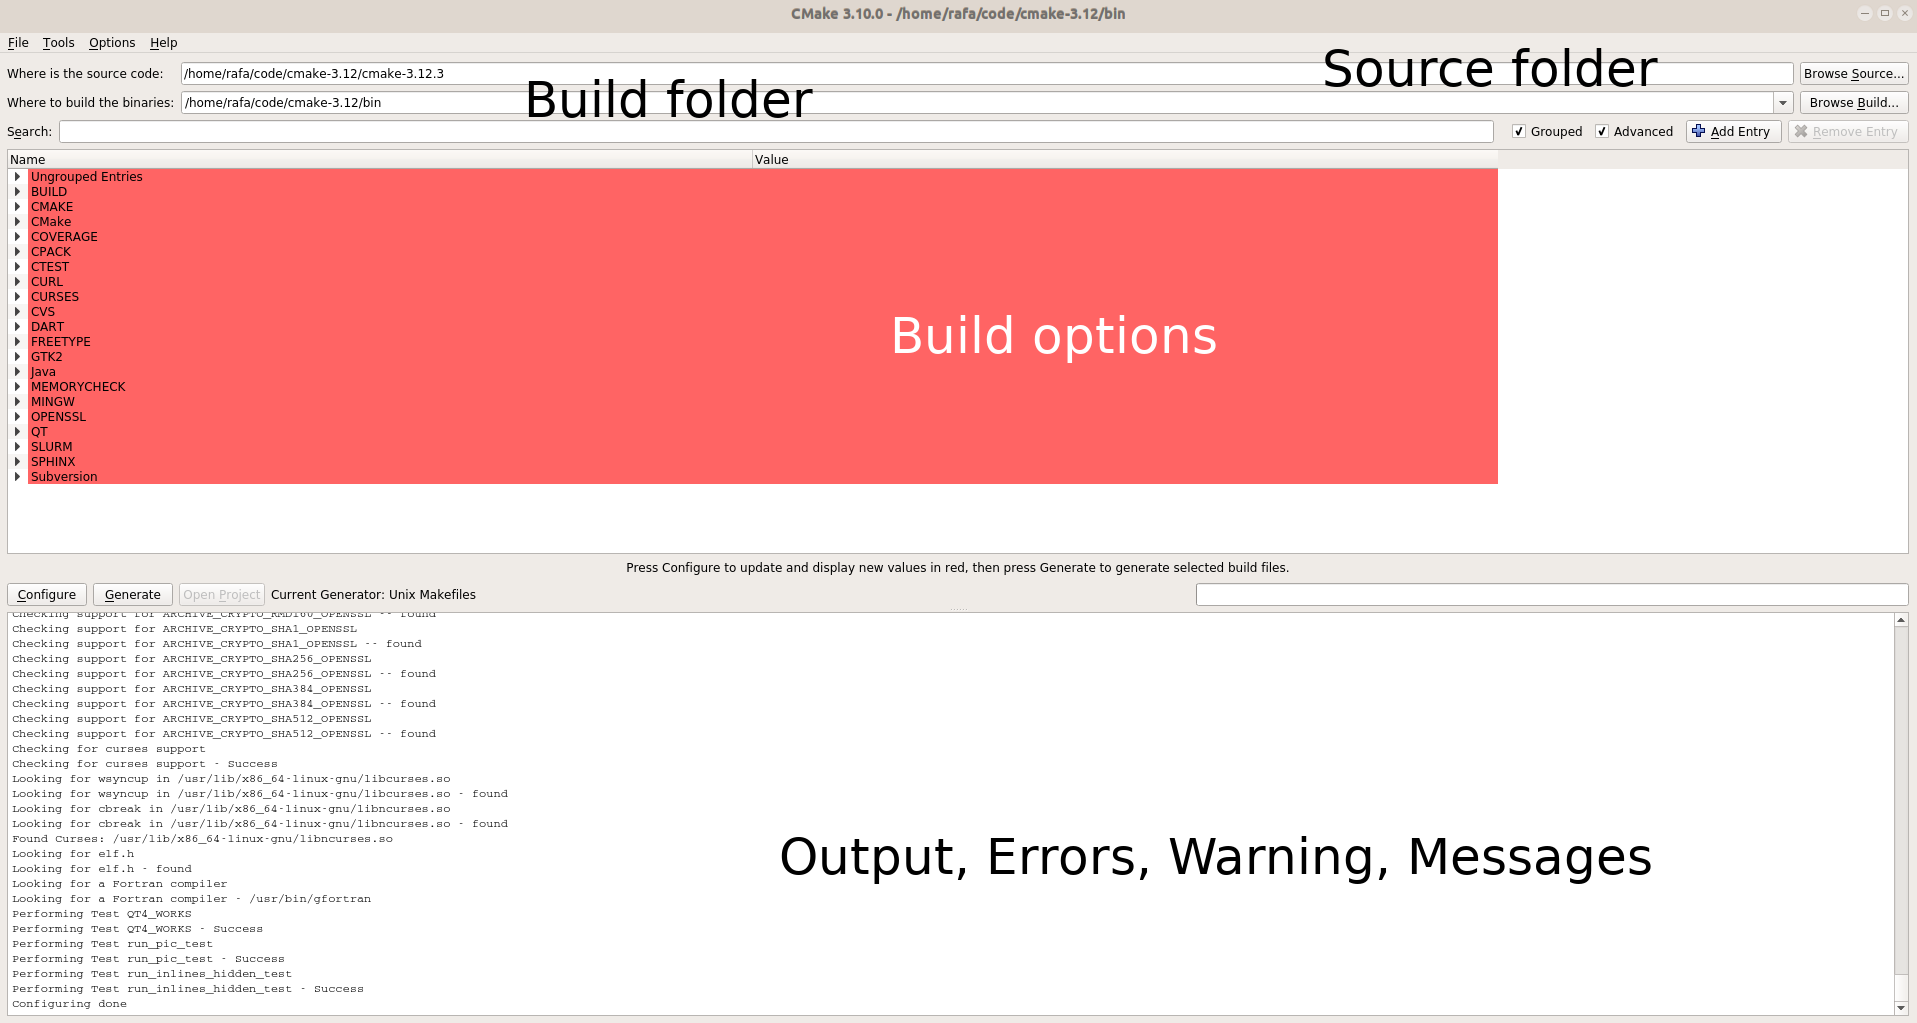
\includegraphics[width=\textwidth]{img/cmake-gui.png}
  \end{center}

\end{frame}

\begin{frame}[fragile]
  \frametitle{Advanced CMake Example}

    \begin{itemize}
      \item Multiple source folders
      \item Add a user defined library  
      \item Search for third-party libraries
    \end{itemize}

  \begin{columns}
    \column{0.5 \textwidth} {
      \begin{center}
        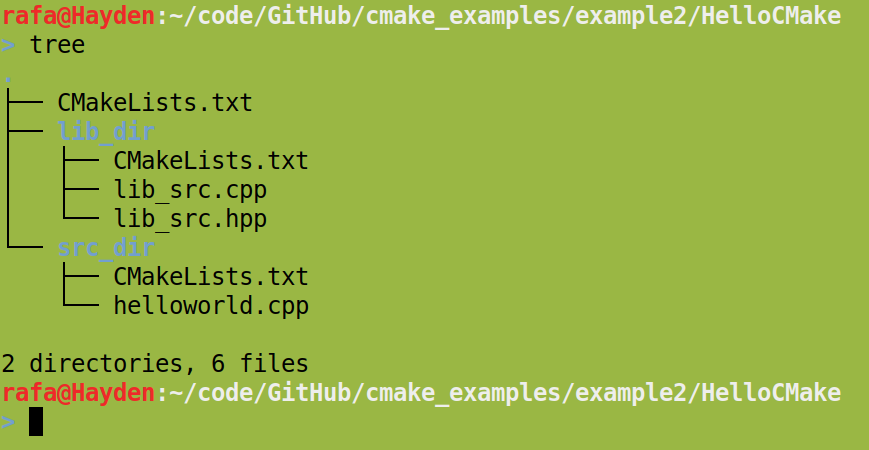
\includegraphics[width=1.0 \textwidth]{img/adv-cmake-dir.png}
      \end{center}
    }
    \column{0.5 \textwidth} {
      \begin{center}
        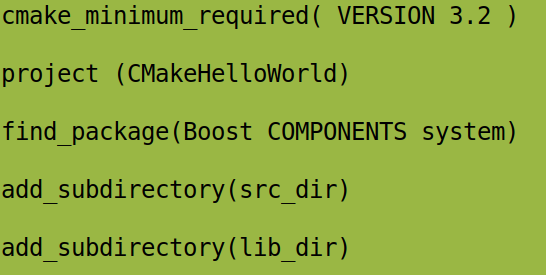
\includegraphics[width=1.0 \textwidth]{img/adv-cmake-code.png}
      \end{center}
    }
\end{columns}

\end{frame}

\begin{frame}[fragile]
  \frametitle{Building a custom library}
  \begin{block}{The lib\_dir CMakeLists.txt}
\begin{verbatim}
set (LIB_SOURCE lib_src.cpp lib_src.hpp)

add_library(hello_lib ${LIB_SOURCE}) 

target_compile_definitions(hello_lib PRIVATE FOO=1)

target_include_directories(hello_lib PUBLIC .)
\end{verbatim}
  \end{block}

\begin{itemize}
  \item Set the include paths or include directories
  \item Add defines that can be used by the preprocessor 
\end{itemize}
  
\end{frame}

\begin{frame}[fragile]
\begin{block}{The src\_dir CMakeLists.txt}
\begin{verbatim}
set (MAIN_SOURCE helloworld.cpp)
add_executable(hello_world ${MAIN_SOURCE})
target_compile_options(hello_world PRIVATE -Wall -Wextra)
if (Boost_FOUND)
  target_compile_definitions(hello_world PRIVATE BAR=1 
  WITH_BOOST=1)
  target_include_directories(hello_world PRIVATE 
  ${CMAKE_SOURCE_DIR}/lib_src ${BOOST_INCLUDE_DIRS})
else(Boost_FOUND)
  target_compile_definitions(hello_world PRIVATE BAR=1)
  target_include_directories(hello_world PRIVATE 
  ${CMAKE_SOURCE_DIR}/lib_src)
endif (Boost_FOUND)
target_link_libraries(hello_world hello_lib)
\end{verbatim}
\end{block}

\end{frame}

\begin{frame}
  \frametitle{CMake - Compilation Flags}
  \begin{block}{Settings Compiler Flags}
    \begin{itemize}
      \item Before CMake version 2.8.12 compilation flags were set by:
      \begin{itemize}
        \item Using the global variable \texttt{CMAKE\_<LANG>\_FLAGS\_<CONFIG>}, i.e. \texttt{CMAKE\_C\_FLAGS\_RELEASE}  
        \item The command \texttt{add\_compile\_options}
      \end{itemize}
    \item Not recommended anymore, \texttt{CMAKE\_<LANG>\_FLAGS\_<CONFIG>} is global
    \item Error prone and 'messy' if you have different targets that require different compilation flags
    \item Since CMake version 2.8.12 it is recommended to use \texttt{target\_compile\_options} sets flags for each individual target
    \item The optimization level is automatically set by CMake when setting the build type:
      \begin{itemize}
        \item \texttt{CMAKE\_BUILD\_TYPE}=Release $\Longrightarrow$ "-O3"
        \item \texttt{CMAKE\_BUILD\_TYPE}=Debug $\Longrightarrow$ "-g"
      \end{itemize}
    \end{itemize}
  \end{block}
\end{frame}

\begin{frame}
  \frametitle{CMake Find Modules}

    \begin{itemize}
      \item CMake has a set of \textbf{CMake modules} to find common third-party libraries
      \item User can provide additional \textbf{CMake modules} to locate libraries 
      \item A \textbf{CMake module} is a *.cmake file written in the CMake language 
      \item Naming convention for module files: \texttt{FindLIBRARY.cmake} 
      \item A custom module needs to be added to the module path 
      \item Module by convention set variables:
    \begin{itemize}
      \item myLibrary\_FOUND: was the library found or not 
      \item myLibrary\_INCLUDE\_DIRS: the include directories of the library  
      \item myLibrary\_LIBRARY\_DIRS: the directories where the libraries are located  
      \item myLibrary\_LIBRARIES: the path to libraries  
      \item ... (see CMake reference on modules)  
    \end{itemize}
    \end{itemize}

\end{frame}

\begin{frame}

  \frametitle{External Projects}
  \begin{itemize}
    \item When libraries are not available on a particular there is still the option to build them from source
    \item Third-party projects/libraries that use CMake can generally be easily integrated
    \item Options:
    \begin{itemize}
      \item Add the library into the project source tree and add it via the command \texttt{add\_subdirectory(lib-dir)}
      \item Use the \texttt{ExternalProject\_Add()} function
    \end{itemize}
    \item About \texttt{ExternalProject\_Add()}:  
    \begin{itemize}
      \item Creates an external target that is not affected by the state of the CMake variables of the main project
      \item Performs the steps: download (from a repo), update, configure, build and install
      \item After the install step the library is ready for use in the main project
    \end{itemize}
  \end{itemize}

\end{frame}

\begin{frame}

  \frametitle{CTest and CDash Overview}

    \begin{itemize}
      \item CTest component allows you define test cases from your CMake targets
      \item CTest defines different test configurations i.e. nightly, experimental, continuous
      \item Execution of a CTest case: update (from repo), configure, build, run, submission to CDash
      \item CDash is a dashboard web application that displays your test results
      \item CDash uses the web technologies:
      \begin{itemize}
        \item Apache server
        \item MySQL database   
        \item PHP
        \item AngularJS
      \end{itemize}
      \item With sufficient knowledge of these technologies CDash can be customized
      \item CTest \keyword{notes} (JSON) can be submitted to make CDash display custom data
    \end{itemize}

\end{frame}

\begin{frame}[plain]
  \begin{center}
    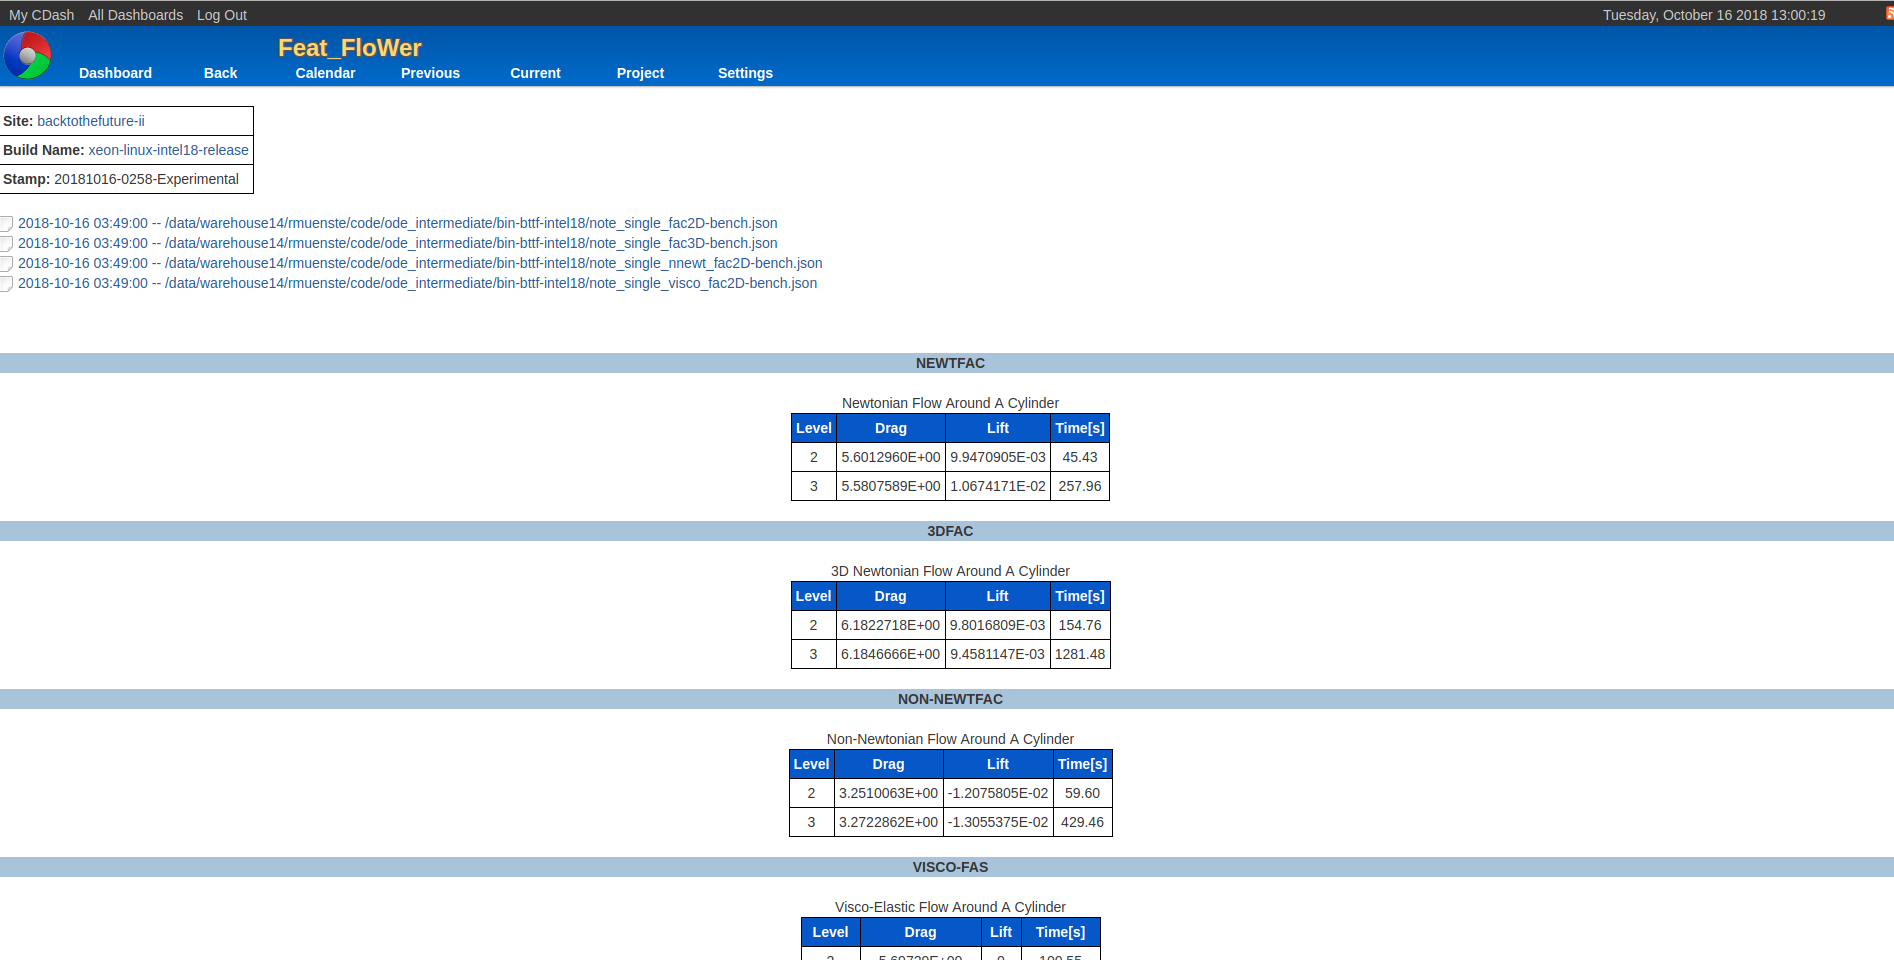
\includegraphics[width=\textwidth]{img/CDASH1.png}
  \end{center}
\end{frame}

\begin{frame}[plain]
  \begin{center}
    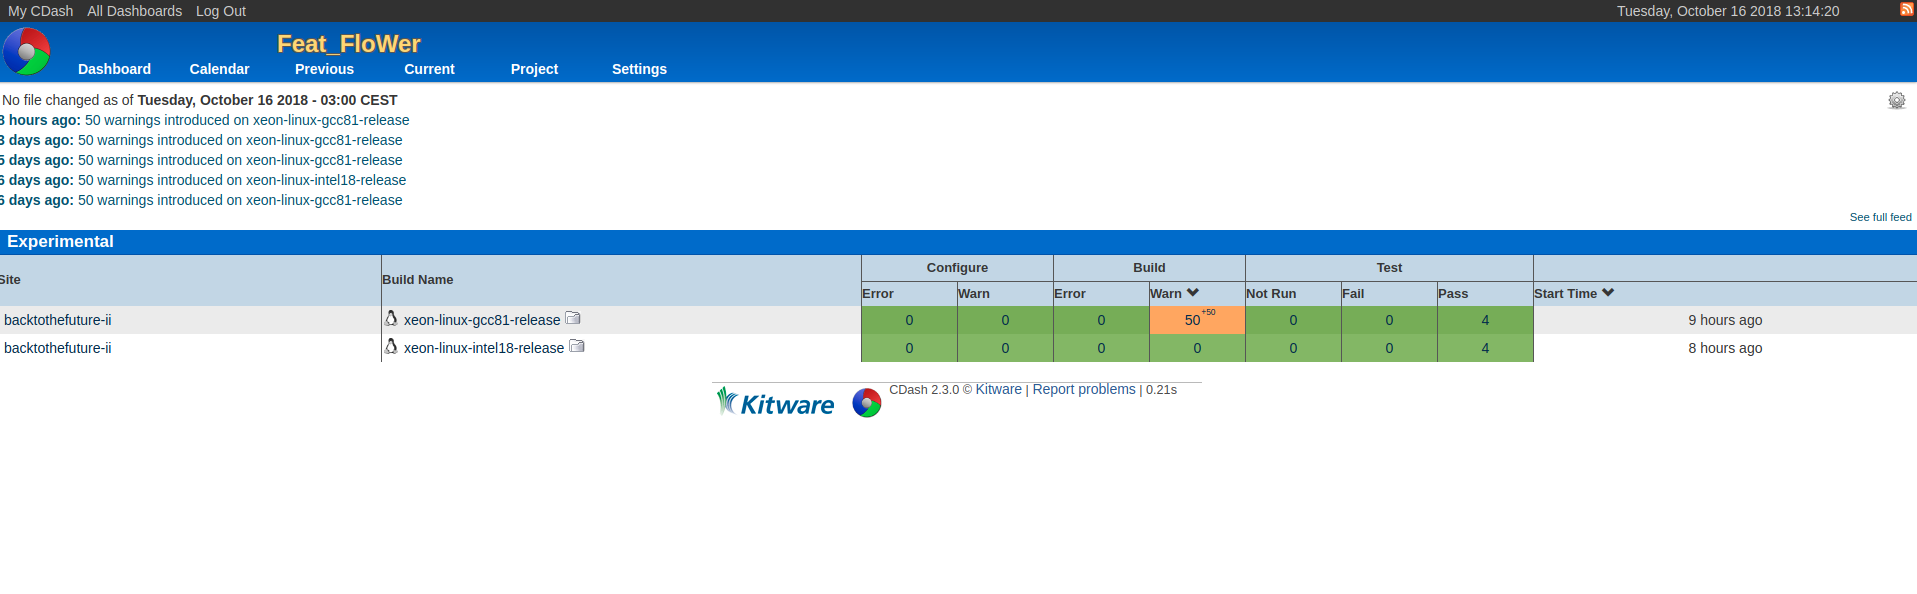
\includegraphics[width=\textwidth]{img/CDASH2.png}
  \end{center}
\end{frame}

\begin{frame}[squeeze]

  \frametitle{Additional CMake Resources}

  \begin{itemize}
      \item Official Kitware CMake language reference:\\
        \url{https://cmake.org/cmake/help/v3.12/manual/cmake-language.7.html}
      \item Short, but very precise overview of the language (recommended):\\
        \url{https://preshing.com/20170522/learn-cmakes-scripting-language-in-15-minutes/}
      \item 'Modern CMake' slides:\\
        \url{https://www.slideshare.net/DanielPfeifer1/cmake-48475415}
      \item A bit old, but free and still valid:\\
        \url{http://www.elpauer.org/stuff/learning_cmake.pdf}
      \item Mastering CMake 3.1 by Kitware:\\
        \url{https://blog.kitware.com/mastering-cmake-is-now-available-on-amazon/}
  \end{itemize}

\end{frame}

